\documentclass{article}

\usepackage{tikz}
\usetikzlibrary{arrows.meta,decorations.pathmorphing,backgrounds,positioning,fit,petri}

\begin{document}

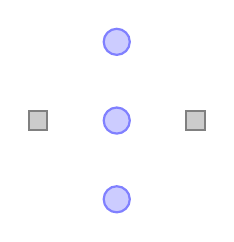
\begin{tikzpicture}
  [place/.style={circle,draw=blue!50,fill=blue!20,thick},
   transition/.style={rectangle,draw=black!50,fill=black!20,thick}]
  \node at ( 0,2) [place] {};
  \node at ( 0,1) [place] {};
  \node at ( 0,0) [place] {};
  \node at ( 1,1) [transition] {};
  \node at (-1,1) [transition] {};
\end{tikzpicture}

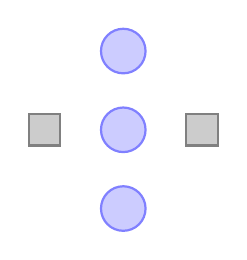
\begin{tikzpicture}
  [inner sep=2mm,
   place/.style={circle,draw=blue!50,fill=blue!20,thick},
   transition/.style={rectangle,draw=black!50,fill=black!20,thick}]
  \node at ( 0,2) [place] {};
  \node at ( 0,1) [place] {};
  \node at ( 0,0) [place] {};
  \node at ( 1,1) [transition] {};
  \node at (-1,1) [transition] {};
\end{tikzpicture}

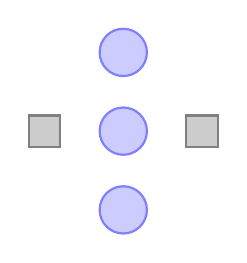
\begin{tikzpicture}
  [place/.style={circle,draw=blue!50,fill=blue!20,thick,
                 inner sep=0pt,minimum size=6mm},
   transition/.style={rectangle,draw=black!50,fill=black!20,thick,
                      inner sep=0pt,minimum size=4mm}]
  \node at ( 0,2) [place] {};
  \node at ( 0,1) [place] {};
  \node at ( 0,0) [place] {};
  \node at ( 1,1) [transition] {};
  \node at (-1,1) [transition] {};
\end{tikzpicture}

\begin{tikzpicture}
  \node[place]      (waiting)                            {};
  \node[place]      (critical)       [below=of waiting]  {};
  \node[place]      (semaphore)      [below=of critical] {};
  \node[transition] (leave critical) [right=of critical] {};
  \node[transition] (enter critical) [left=of critical]  {};
  \node[red,above] at (semaphore.north) {$s\le 3A$};
\end{tikzpicture}

\begin{tikzpicture}
  \node[place]      (waiting)                            {};
  \node[place]      (critical)       [below=of waiting]  {};
  \node[place]      (semaphore)      [below=of critical,
                                      label=above:$s\le3$] {};
  \node[transition] (leave critical) [right=of critical] {};
  \node[transition] (enter critical) [left=of critical]  {};
\end{tikzpicture}

\tikz
  \node [circle,draw,label=60:$60^\circ$,label=below:$-90^\circ$] {my circle};

\begin{tikzpicture}[every label/.style={red}]
  \node[place]      (waiting)                            {};
  \node[place]      (critical)       [below=of waiting]  {};
  \node[place]      (semaphore)      [below=of critical,
                                      label={[red]above:$s\le3$}] {};
  \node[transition] (leave critical) [right=of critical] {};
  \node[transition] (enter critical) [left=of critical]  {};
\end{tikzpicture}

\begin{tikzpicture}
  \node[place]      (waiting)                            {};
  \node[place]      (critical)       [below=of waiting]  {};
  \node[place]      (semaphore)      [below=of critical] {};
  \node[transition] (leave critical) [right=of critical] {};
  \node[transition] (enter critical) [left=of critical]  {};
  \draw [->] (enter critical) -- (critical);
  \draw [->] (waiting) .. controls +(left:8mm) and +(up:8mm)
                            .. (enter critical);
\end{tikzpicture}

\begin{tikzpicture}
  \node[place]      (waiting)                            {};
  \node[place]      (critical)       [below=of waiting]  {};
  \node[place]      (semaphore)      [below=of critical] {};
  \node[transition] (leave critical) [right=of critical] {};
  \node[transition] (enter critical) [left=of critical]  {};
  \draw [->] (enter critical) to (critical);
  \draw [->] (waiting) to [out=180,in=90] (enter critical);
\end{tikzpicture}

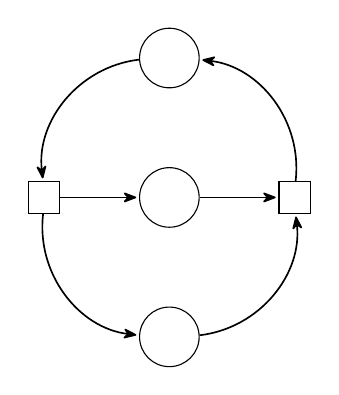
\begin{tikzpicture}
  [bend angle=45,
   pre/.style={<-,shorten <=1pt,>={Stealth[round]},semithick},
   post/.style={->,shorten >=1pt,>={Stealth[round]},semithick}]

  \node[place]      (waiting)                            {};
  \node[place]      (critical)       [below=of waiting]  {};
  \node[place]      (semaphore)      [below=of critical] {};

  \node[transition] (leave critical) [right=of critical] {}
    edge [pre]             (critical)
    edge [post,bend right] (waiting)
    edge [pre, bend left]  (semaphore);
  \node[transition] (enter critical) [left=of critical]  {}
    edge [post]            (critical)
    edge [pre, bend left]  (waiting)
    edge [post,bend right] (semaphore);
\end{tikzpicture}

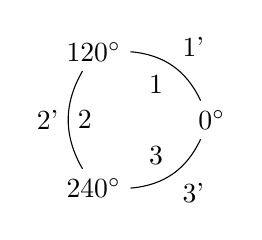
\begin{tikzpicture}[auto,bend right]
  \node (a) at (0:1) {$0^\circ$};
  \node (b) at (120:1) {$120^\circ$};
  \node (c) at (240:1) {$240^\circ$};

  \draw (a) to node {1} node [swap] {1'} (b)
        (b) to node {2} node [swap] {2'} (c)
        (c) to node {3} node [swap] {3'} (a);
\end{tikzpicture}

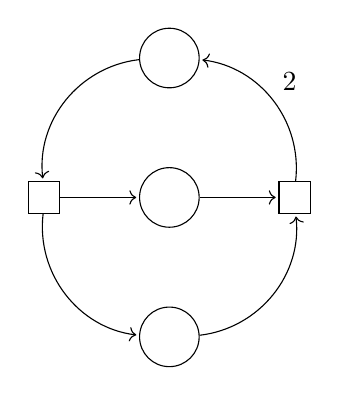
\begin{tikzpicture}[bend angle=45]
  \node[place]      (waiting)                            {};
  \node[place]      (critical)       [below=of waiting]  {};
  \node[place]      (semaphore)      [below=of critical] {};

  \node[transition] (leave critical) [right=of critical] {}
    edge [pre]                                 (critical)
    edge [post,bend right] node[auto,swap] {2} (waiting)
    edge [pre, bend left]                      (semaphore);
  \node[transition] (enter critical) [left=of critical]  {}
    edge [post]                                (critical)
    edge [pre, bend left]                      (waiting)
    edge [post,bend right]                     (semaphore);
\end{tikzpicture}

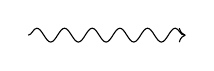
\begin{tikzpicture}
  \draw [->,decorate,decoration=snake] (0,0) -- (2,0);
\end{tikzpicture}

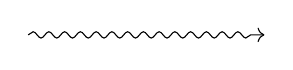
\begin{tikzpicture}
  \draw [->,decorate,
     decoration={snake,amplitude=.4mm,segment length=2mm,post length=1mm}]
    (0,0) -- (3,0);
\end{tikzpicture}

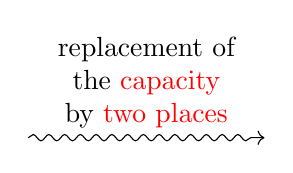
\begin{tikzpicture}
  \draw [->,decorate,
      decoration={snake,amplitude=.4mm,segment length=2mm,post length=1mm}]
    (0,0) -- (3,0)
    node [above,align=center,midway]
    {
      replacement of\\
      the \textcolor{red}{capacity}\\
      by \textcolor{red}{two places}
    };
\end{tikzpicture}

\usetikzlibrary {decorations.pathmorphing}
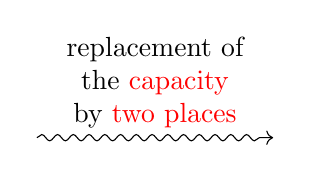
\begin{tikzpicture}
  \draw [->,decorate,
      decoration={snake,amplitude=.4mm,segment length=2mm,post length=1mm}]
    (0,0) -- (3,0)
    node [above,text width=3cm,align=center,midway]
    {
      replacement of the \textcolor{red}{capacity} by
      \textcolor{red}{two places}
    };
\end{tikzpicture}

\usetikzlibrary {arrows.meta,backgrounds,fit,positioning}
% Styles as before
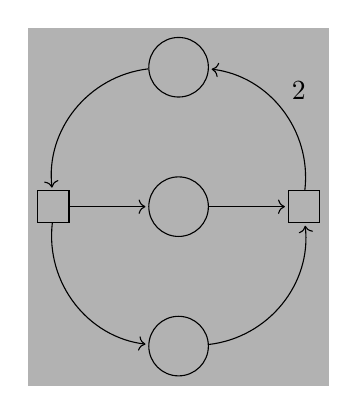
\begin{tikzpicture}[bend angle=45]
  \node[place]      (waiting)                            {};
  \node[place]      (critical)       [below=of waiting]  {};
  \node[place]      (semaphore)      [below=of critical] {};

  \node[transition] (leave critical) [right=of critical] {}
    edge [pre]                                 (critical)
    edge [post,bend right] node[auto,swap] {2} (waiting)
    edge [pre, bend left]                      (semaphore);
  \node[transition] (enter critical) [left=of critical]  {}
    edge [post]                                (critical)
    edge [pre, bend left]                      (waiting)
    edge [post,bend right]                     (semaphore);

  \begin{scope}[on background layer]
    \node [fill=black!30,fit=(waiting) (critical) (semaphore)
             (leave critical) (enter critical)] {};
  \end{scope}
\end{tikzpicture}

\end{document}
